% Created by tikzDevice version 0.12.6 on 2025-04-03 14:58:44
% !TEX encoding = UTF-8 Unicode
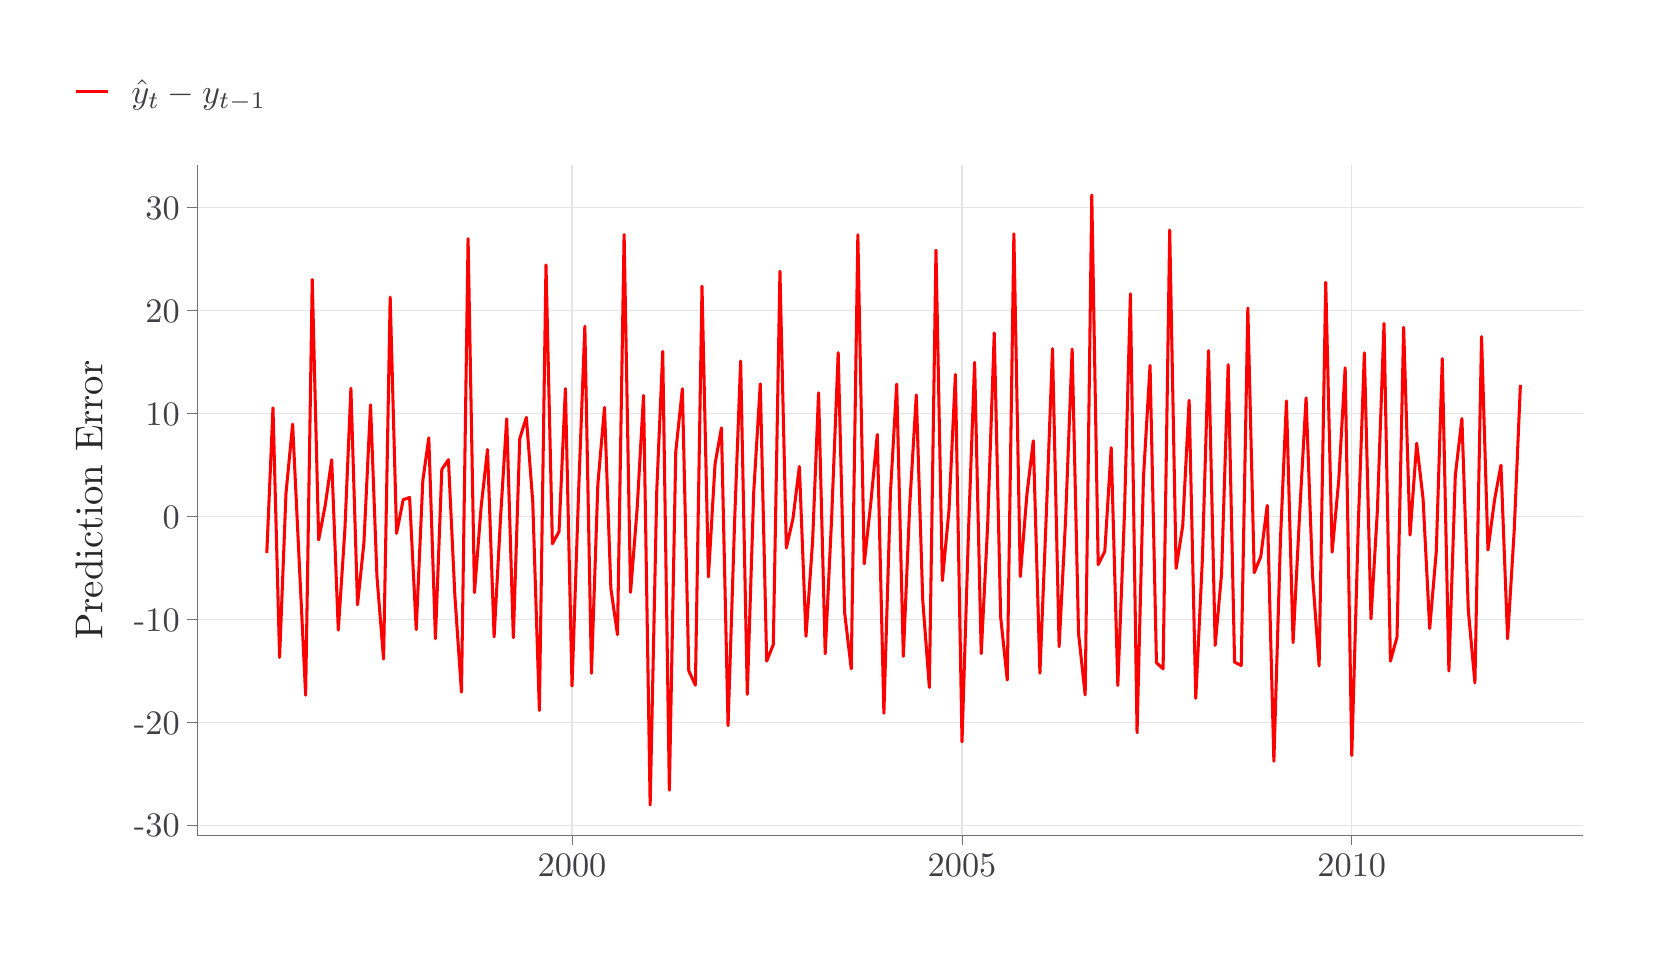
\begin{tikzpicture}[x=1pt,y=1pt]
\definecolor{fillColor}{RGB}{255,255,255}
\path[use as bounding box,fill=fillColor] (0,0) rectangle (578.16,325.21);
\begin{scope}
\path[clip] (  0.00,  0.00) rectangle (578.16,325.21);
\definecolor{drawColor}{RGB}{255,255,255}

\path[draw=drawColor,line width= 0.7pt,line join=round,line cap=round,fill=fillColor] (  0.00,  0.00) rectangle (578.16,325.21);
\end{scope}
\begin{scope}
\path[clip] ( 61.25, 33.29) rectangle (562.16,275.76);
\definecolor{drawColor}{RGB}{255,255,255}
\definecolor{fillColor}{RGB}{255,255,255}

\path[draw=drawColor,line width= 0.7pt,line join=round,line cap=round,fill=fillColor] ( 61.25, 33.29) rectangle (562.16,275.76);
\definecolor{drawColor}{RGB}{228,228,231}

\path[draw=drawColor,line width= 0.4pt,line join=round] ( 61.25, 37.05) --
	(562.16, 37.05);

\path[draw=drawColor,line width= 0.4pt,line join=round] ( 61.25, 74.25) --
	(562.16, 74.25);

\path[draw=drawColor,line width= 0.4pt,line join=round] ( 61.25,111.45) --
	(562.16,111.45);

\path[draw=drawColor,line width= 0.4pt,line join=round] ( 61.25,148.65) --
	(562.16,148.65);

\path[draw=drawColor,line width= 0.4pt,line join=round] ( 61.25,185.84) --
	(562.16,185.84);

\path[draw=drawColor,line width= 0.4pt,line join=round] ( 61.25,223.04) --
	(562.16,223.04);

\path[draw=drawColor,line width= 0.4pt,line join=round] ( 61.25,260.24) --
	(562.16,260.24);

\path[draw=drawColor,line width= 0.4pt,line join=round] (196.70, 33.29) --
	(196.70,275.76);

\path[draw=drawColor,line width= 0.4pt,line join=round] (337.62, 33.29) --
	(337.62,275.76);

\path[draw=drawColor,line width= 0.4pt,line join=round] (478.46, 33.29) --
	(478.46,275.76);
\definecolor{drawColor}{RGB}{255,0,0}

\path[draw=drawColor,line width= 1.1pt,line join=round] ( 86.41,135.37) --
	( 88.64,187.85) --
	( 91.03, 97.61) --
	( 93.35,157.05) --
	( 95.74,181.94) --
	( 98.05,133.73) --
	(100.44, 83.96) --
	(102.83,234.20) --
	(105.15,140.09) --
	(107.54,152.74) --
	(109.85,169.07) --
	(112.24,107.51) --
	(114.64,144.11) --
	(116.80,194.92) --
	(119.19,116.69) --
	(121.50,139.01) --
	(123.89,188.93) --
	(126.21,126.92) --
	(128.60, 97.05) --
	(130.99,227.84) --
	(133.30,142.47) --
	(135.69,154.64) --
	(138.01,155.45) --
	(140.40,107.73) --
	(142.79,161.63) --
	(144.95,176.99) --
	(147.34,104.42) --
	(149.65,165.57) --
	(152.04,169.10) --
	(154.36,120.08) --
	(156.75, 85.08) --
	(159.14,248.97) --
	(161.45,121.08) --
	(163.84,151.92) --
	(166.16,172.79) --
	(168.55,105.09) --
	(170.94,149.32) --
	(173.10,183.87) --
	(175.49,104.79) --
	(177.81,176.69) --
	(180.20,184.39) --
	(182.51,153.82) --
	(184.90, 78.49) --
	(187.29,239.52) --
	(189.61,138.71) --
	(192.00,143.10) --
	(194.31,194.77) --
	(196.70, 87.27) --
	(199.09,157.83) --
	(201.33,217.31) --
	(203.72, 91.92) --
	(206.03,160.14) --
	(208.43,187.96) --
	(210.74,122.53) --
	(213.13,105.87) --
	(215.52,250.49) --
	(217.84,121.19) --
	(220.23,151.40) --
	(222.54,192.35) --
	(224.93, 44.31) --
	(227.32,157.91) --
	(229.48,208.20) --
	(231.87, 49.70) --
	(234.19,172.04) --
	(236.58,194.73) --
	(238.89, 92.81) --
	(241.28, 87.61) --
	(243.67,231.78) --
	(245.99,126.74) --
	(248.38,167.54) --
	(250.69,180.60) --
	(253.08, 73.02) --
	(255.48,147.72) --
	(257.63,204.74) --
	(260.03, 84.29) --
	(262.34,157.13) --
	(264.73,196.52) --
	(267.04, 96.31) --
	(269.44,102.34) --
	(271.83,237.18) --
	(274.14,137.19) --
	(276.53,147.75) --
	(278.85,166.65) --
	(281.24,105.27) --
	(283.63,139.61) --
	(285.79,193.25) --
	(288.18, 98.95) --
	(290.49,147.57) --
	(292.88,207.75) --
	(295.20,113.90) --
	(297.59, 93.52) --
	(299.98,250.38) --
	(302.29,131.50) --
	(304.68,153.63) --
	(307.00,178.18) --
	(309.39, 77.52) --
	(311.78,157.54) --
	(314.02,196.41) --
	(316.41, 98.02) --
	(318.72,152.59) --
	(321.11,192.50) --
	(323.43,118.37) --
	(325.82, 86.79) --
	(328.21,244.80) --
	(330.52,125.40) --
	(332.91,150.84) --
	(335.23,199.90) --
	(337.62, 67.18) --
	(340.01,144.59) --
	(342.17,204.29) --
	(344.56, 99.02) --
	(346.87,145.08) --
	(349.27,214.93) --
	(351.58,112.27) --
	(353.97, 89.50) --
	(356.36,250.72) --
	(358.68,126.89) --
	(361.07,156.53) --
	(363.38,175.91) --
	(365.77, 91.96) --
	(368.16,151.25) --
	(370.32,209.20) --
	(372.71,101.55) --
	(375.03,147.12) --
	(377.42,209.09) --
	(379.73,106.32) --
	(382.12, 84.11) --
	(384.51,264.74) --
	(386.83,131.20) --
	(389.22,136.00) --
	(391.53,173.42) --
	(393.92, 87.49) --
	(396.31,149.28) --
	(398.47,229.07) --
	(400.87, 70.46) --
	(403.18,162.60) --
	(405.57,203.18) --
	(407.88, 95.75) --
	(410.28, 93.52) --
	(412.67,252.09) --
	(414.98,129.79) --
	(417.37,145.15) --
	(419.69,190.57) --
	(422.08, 82.84) --
	(424.47,132.95) --
	(426.70,208.50) --
	(429.10,102.00) --
	(431.41,127.89) --
	(433.80,203.44) --
	(436.11, 95.94) --
	(438.51, 94.75) --
	(440.90,223.90) --
	(443.21,128.26) --
	(445.60,134.14) --
	(447.91,152.59) --
	(450.31, 60.12) --
	(452.70,140.50) --
	(454.86,190.34) --
	(457.25,103.01) --
	(459.56,148.53) --
	(461.95,191.46) --
	(464.27,127.41) --
	(466.66, 94.56) --
	(469.05,233.20) --
	(471.36,135.66) --
	(473.75,161.63) --
	(476.07,202.32) --
	(478.46, 62.20) --
	(480.85,146.64) --
	(483.01,207.72) --
	(485.40,111.60) --
	(487.71,150.65) --
	(490.11,218.35) --
	(492.42, 96.31) --
	(494.81,105.01) --
	(497.20,216.94) --
	(499.51,141.88) --
	(501.91,175.02) --
	(504.22,155.01) --
	(506.61,108.06) --
	(509.00,135.96) --
	(511.16,205.63) --
	(513.55, 92.74) --
	(515.87,163.34) --
	(518.26,183.98) --
	(520.57,114.69) --
	(522.96, 88.42) --
	(525.35,213.59) --
	(527.67,136.48) --
	(530.06,154.60) --
	(532.37,167.13) --
	(534.76,104.38) --
	(537.15,143.44) --
	(539.39,196.11);
\end{scope}
\begin{scope}
\path[clip] (  0.00,  0.00) rectangle (578.16,325.21);
\definecolor{drawColor}{RGB}{113,113,122}

\path[draw=drawColor,line width= 0.3pt,line join=round] ( 61.25, 33.29) --
	( 61.25,275.76);
\end{scope}
\begin{scope}
\path[clip] (  0.00,  0.00) rectangle (578.16,325.21);
\definecolor{drawColor}{RGB}{63,63,70}

\node[text=drawColor,anchor=base east,inner sep=0pt, outer sep=0pt, scale=  1.24] at ( 54.95, 32.77) {-30};

\node[text=drawColor,anchor=base east,inner sep=0pt, outer sep=0pt, scale=  1.24] at ( 54.95, 69.97) {-20};

\node[text=drawColor,anchor=base east,inner sep=0pt, outer sep=0pt, scale=  1.24] at ( 54.95,107.17) {-10};

\node[text=drawColor,anchor=base east,inner sep=0pt, outer sep=0pt, scale=  1.24] at ( 54.95,144.36) {0};

\node[text=drawColor,anchor=base east,inner sep=0pt, outer sep=0pt, scale=  1.24] at ( 54.95,181.56) {10};

\node[text=drawColor,anchor=base east,inner sep=0pt, outer sep=0pt, scale=  1.24] at ( 54.95,218.76) {20};

\node[text=drawColor,anchor=base east,inner sep=0pt, outer sep=0pt, scale=  1.24] at ( 54.95,255.95) {30};
\end{scope}
\begin{scope}
\path[clip] (  0.00,  0.00) rectangle (578.16,325.21);
\definecolor{drawColor}{RGB}{113,113,122}

\path[draw=drawColor,line width= 0.3pt,line join=round] ( 57.75, 37.05) --
	( 61.25, 37.05);

\path[draw=drawColor,line width= 0.3pt,line join=round] ( 57.75, 74.25) --
	( 61.25, 74.25);

\path[draw=drawColor,line width= 0.3pt,line join=round] ( 57.75,111.45) --
	( 61.25,111.45);

\path[draw=drawColor,line width= 0.3pt,line join=round] ( 57.75,148.65) --
	( 61.25,148.65);

\path[draw=drawColor,line width= 0.3pt,line join=round] ( 57.75,185.84) --
	( 61.25,185.84);

\path[draw=drawColor,line width= 0.3pt,line join=round] ( 57.75,223.04) --
	( 61.25,223.04);

\path[draw=drawColor,line width= 0.3pt,line join=round] ( 57.75,260.24) --
	( 61.25,260.24);
\end{scope}
\begin{scope}
\path[clip] (  0.00,  0.00) rectangle (578.16,325.21);
\definecolor{drawColor}{RGB}{113,113,122}

\path[draw=drawColor,line width= 0.3pt,line join=round] ( 61.25, 33.29) --
	(562.16, 33.29);
\end{scope}
\begin{scope}
\path[clip] (  0.00,  0.00) rectangle (578.16,325.21);
\definecolor{drawColor}{RGB}{113,113,122}

\path[draw=drawColor,line width= 0.3pt,line join=round] (196.70, 29.79) --
	(196.70, 33.29);

\path[draw=drawColor,line width= 0.3pt,line join=round] (337.62, 29.79) --
	(337.62, 33.29);

\path[draw=drawColor,line width= 0.3pt,line join=round] (478.46, 29.79) --
	(478.46, 33.29);
\end{scope}
\begin{scope}
\path[clip] (  0.00,  0.00) rectangle (578.16,325.21);
\definecolor{drawColor}{RGB}{63,63,70}

\node[text=drawColor,anchor=base,inner sep=0pt, outer sep=0pt, scale=  1.24] at (196.70, 18.42) {2000};

\node[text=drawColor,anchor=base,inner sep=0pt, outer sep=0pt, scale=  1.24] at (337.62, 18.42) {2005};

\node[text=drawColor,anchor=base,inner sep=0pt, outer sep=0pt, scale=  1.24] at (478.46, 18.42) {2010};
\end{scope}
\begin{scope}
\path[clip] (  0.00,  0.00) rectangle (578.16,325.21);
\definecolor{drawColor}{RGB}{39,39,42}

\node[text=drawColor,rotate= 90.00,anchor=base,inner sep=0pt, outer sep=0pt, scale=  1.40] at ( 27.00,154.52) {Prediction Error};
\end{scope}
\begin{scope}
\path[clip] (  0.00,  0.00) rectangle (578.16,325.21);
\definecolor{drawColor}{RGB}{255,255,255}
\definecolor{fillColor}{RGB}{255,255,255}

\path[draw=drawColor,line width= 0.7pt,line join=round,line cap=round,fill=fillColor] ( 16.00,289.76) rectangle ( 86.35,309.22);
\end{scope}
\begin{scope}
\path[clip] (  0.00,  0.00) rectangle (578.16,325.21);
\definecolor{drawColor}{RGB}{255,255,255}
\definecolor{fillColor}{RGB}{255,255,255}

\path[draw=drawColor,line width= 0.7pt,line join=round,line cap=round,fill=fillColor] ( 16.00,294.76) rectangle ( 30.45,309.22);
\end{scope}
\begin{scope}
\path[clip] (  0.00,  0.00) rectangle (578.16,325.21);
\definecolor{drawColor}{RGB}{255,0,0}

\path[draw=drawColor,line width= 1.1pt,line join=round] ( 17.45,301.99) -- ( 29.01,301.99);
\end{scope}
\begin{scope}
\path[clip] (  0.00,  0.00) rectangle (578.16,325.21);
\definecolor{drawColor}{RGB}{63,63,70}

\node[text=drawColor,anchor=base west,inner sep=0pt, outer sep=0pt, scale=  1.24] at ( 37.45,297.70) {$\hat{y}_t - y_{t-1}$};
\end{scope}
\end{tikzpicture}
